\documentclass[border=8pt]{standalone}
\usepackage{tikz}
\usetikzlibrary{arrows.meta,positioning,calc}
\begin{document}
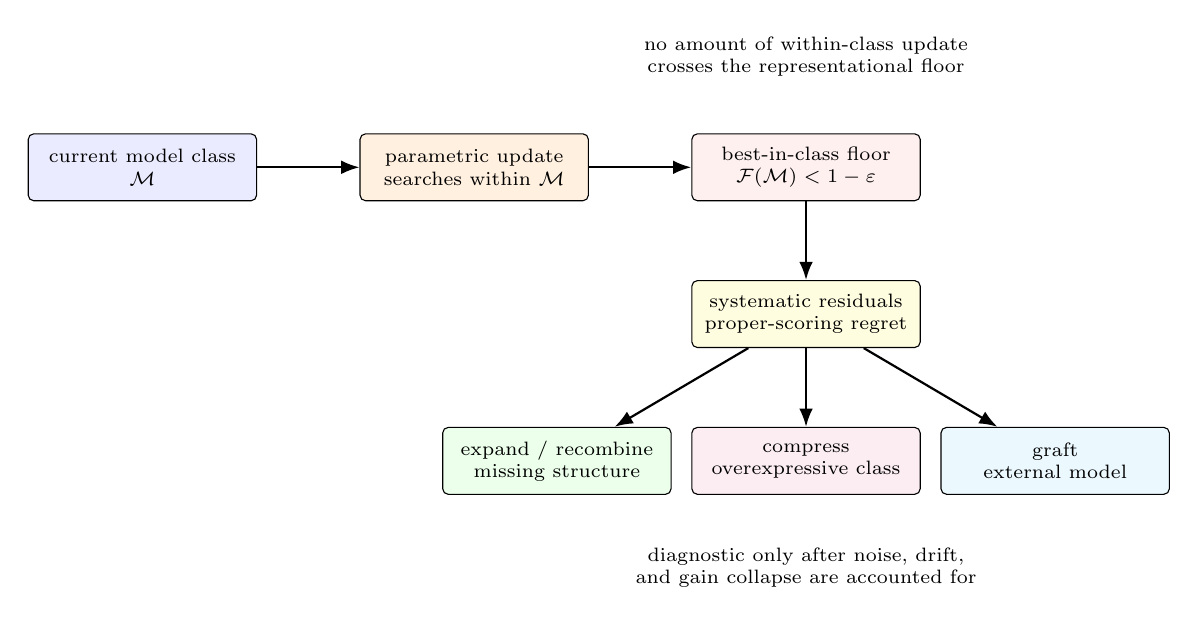
\begin{tikzpicture}[
  box/.style={draw, rounded corners=2pt, align=center, minimum width=2.9cm, minimum height=0.85cm, font=\scriptsize},
  note/.style={align=center, font=\scriptsize},
  arr/.style={-Latex, thick},
  dasharr/.style={-Latex, thick, dashed}
]

\node[box, fill=blue!8] (class) {current model class\\$\mathcal M$};
\node[box, fill=orange!12, right=1.3cm of class] (param) {parametric update\\searches within $\mathcal M$};
\node[box, fill=red!6, right=1.3cm of param] (floor) {best-in-class floor\\$\mathcal F(\mathcal M)<1-\varepsilon$};
\draw[arr] (class) -- (param);
\draw[arr] (param) -- (floor);

\node[box, fill=yellow!12, below=1.0cm of floor] (resid) {systematic residuals\\proper-scoring regret};
\draw[arr] (floor) -- (resid);

\node[box, fill=green!8, below left=1.0cm and 0.25cm of resid] (expand) {expand / recombine\\missing structure};
\node[box, fill=purple!7, below=1.0cm of resid] (compress) {compress\\overexpressive class};
\node[box, fill=cyan!8, below right=1.0cm and 0.25cm of resid] (graft) {graft\\external model};
\draw[arr] (resid) -- (expand);
\draw[arr] (resid) -- (compress);
\draw[arr] (resid) -- (graft);

\node[note, above=0.6cm of floor] {no amount of within-class update\\crosses the representational floor};
\node[note, below=0.55cm of compress] {diagnostic only after noise, drift,\\and gain collapse are accounted for};

\end{tikzpicture}
\end{document}
